
\chapter{Resultados}

\lettrine{E}{n} este capítulo analizaremos los resultados obtenidos en los modelos estudiados, realizando en todos ellos una división de los datos de entrenamiento mediante k-fold, que nos permite comparar los modelos según precisión media.

\section{Corpus de datos}\label{corpus}

\subsection{Corpus TASS}
Se trata de un corpus ofrecido por el TASS \footnote{http://www.sepln.org/workshops/tass/2016/tass2016.php}, taller que se centra en las tareas de análisis de sentimientos y de reputación para el idioma español, organizado como evento satélite en la conferencia anual de la SEPLN (Sociedad Española para el Procesamiento del Lenguaje Natural).

Proponen dos tipos de clasificaciones: una basada en un sistema de 6 clases (Positivo +, Positivo, Neutro, Negativo, Negativo +, None) y otra en 4 clases (Negativo, Neutro, Positivo, None).

Para ello ofrecen un conjunto de 6800 tweets para entrenamiento, que vienen acompañados de una polaridad supervisada que se encontrará dentro del rango de 6 clases anteriormente citado.

\begin{figure}[!ht]
	\centering
	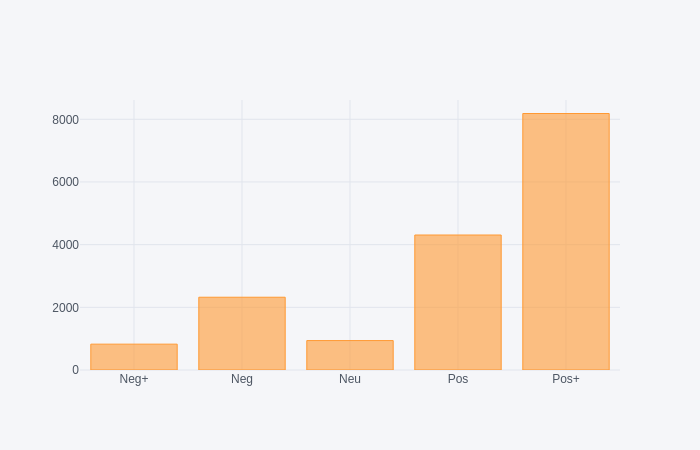
\includegraphics[width=0.75\textwidth]{imaxes/distTass.png}
	\caption{Distribución de la polarización.}
	\label{dist_tass}
\end{figure}

\begin{figure}[!ht]
	\centering
	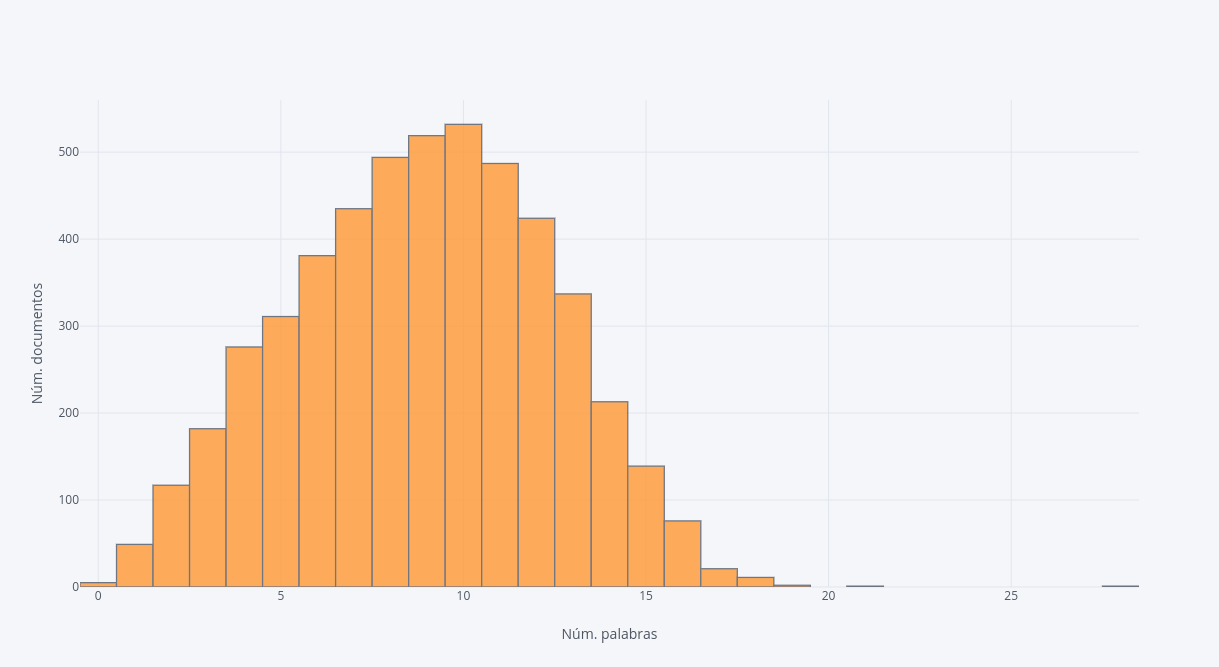
\includegraphics[width=1\textwidth]{imaxes/distTokensTass.png}
	\caption{Histograma de número de palabras por documento.}
	\label{dist_tokes_tass}
\end{figure}

En la figura \ref{dist_tass} se muestra la distribución de polaridades en el corpus TASS, en ella vemos una distribución con tendencia hacia los extremos, sobre todo a las polaridades positivas. Por otro lado la figura \ref{dist_tokes_tass} nos muestra un histograma del número de palabras por documento en el cual vemos que la mayoría de ellos contienen tan sólo 10 o menos palabras, alcanzando un máximo de 28.

Hemos traducido un lexicón de palabras polarizadas del inglés para cruzarlos con los tweets de la colección y comprobar la distribución de las palabras en los mismos, obteniendo los siguientes resultados:

\begin{figure}[H]
	\centering
	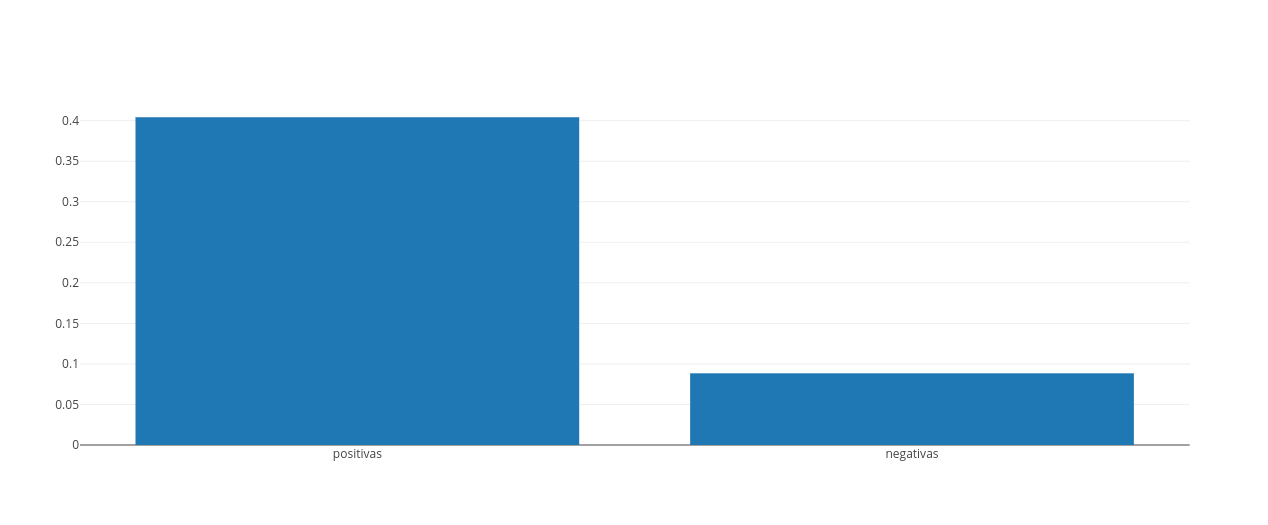
\includegraphics[width=0.75\textwidth]{imaxes/dist_pos_neg.png}
	\caption{Distribución de las palabras polarizadas en tweets positivos}
	\label{dist_pos}
\end{figure}

Como se ve en la figura \ref{dist_pos} los tweets positivos presentan un cantidad notablemente mayor de palabras positivas, por lo que podemos deducir, que la clasificación de estos tweets en su clase debería ser sencilla, si somos capaces de eliminar correctamente todas las palabras que puedan aportar ruido innecesario al modelo.

\begin{figure}[H]
	\centering
	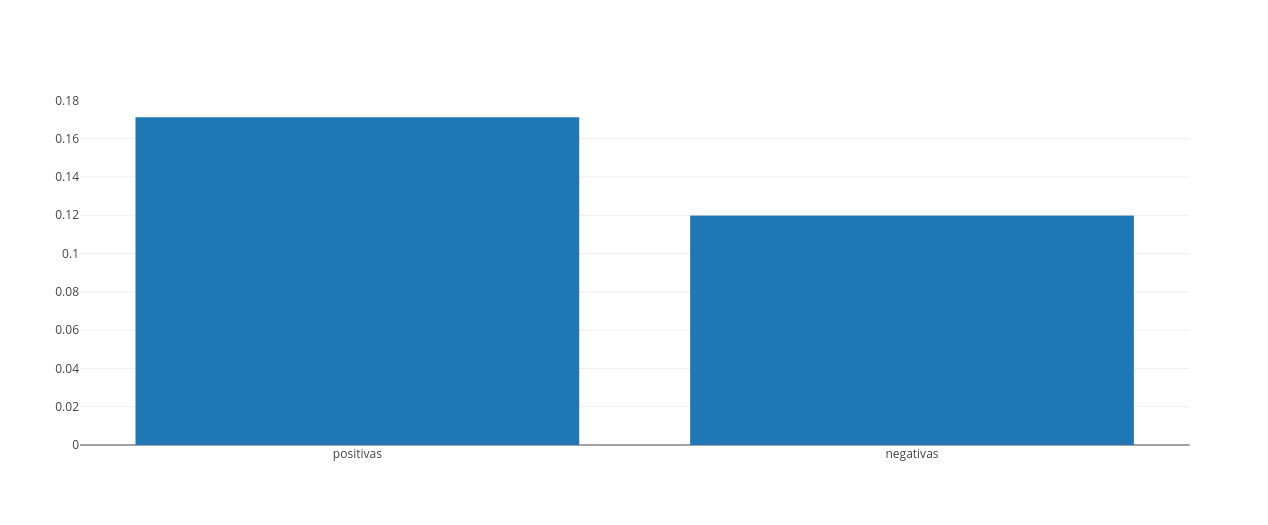
\includegraphics[width=0.75\textwidth]{imaxes/dist_pos_neg_neg.png}
	\caption{Distribución de las palabras polarizadas en tweets negativos}
	\label{dist_neg}
\end{figure}

En el caso de los tweets negativos la gráfica \ref{dist_neg} podemos observar que está más compensada, por lo que será más complicado para el modelo discernir la clase de estos tweets

\begin{figure}[!ht]
	\centering
	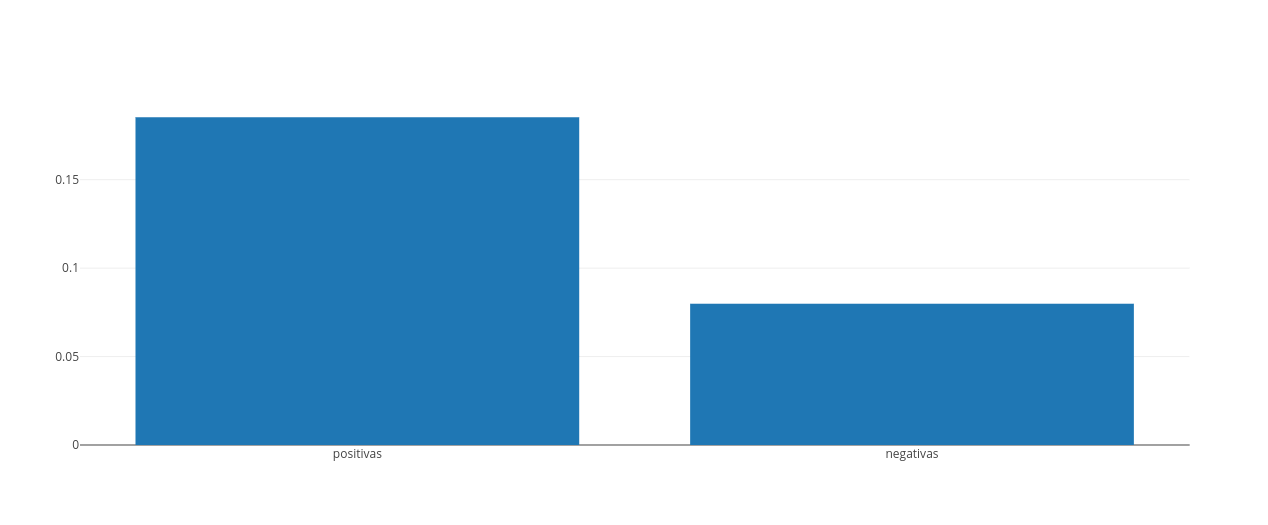
\includegraphics[width=0.75\textwidth]{imaxes/dist_pos_neg_neut.png}
	\caption{Distribución de las palabras polarizadas en tweets neutros}
	\label{dist_neut}
\end{figure}

Para los tweets con clase neutral, se encuentran más palabras positivas que negativas, con lo que es muy probable que estos tweets acaben clasificados en una clase positiva.

Dado este análisis podemos deducir que el modelo de clasificación tendrá facilidad al clasificar los tweets positivos, pero dificultades al clasificar el resto. Esta tendencia del lenguaje a mostrar positividad ya ha sido demostrada por diversos estudios como los propuestos por Kloumann, Isabel M et al. \cite{PoeEL} y Dodds, Peter Sheridan et al. \cite{HulPB}.

\subsection{Corpus Cine}

Ya que en el momento actual no tenemos conocimiento de como van a ser los textos reales del dominio de la aplicación necesitamos probar los modelos contra textos más extensos y escritos de una forma más formal.

Se trata de un corpus descargado de la página MuchoCine.com para el trabajo, con la intención de disponer de un conjunto de documentos más extenso, tanto en número de documentos como en cantidad de palabras por documento (ver fig. \ref{dist_tokes_pelis}).

Estos documentos están clasificados con un sistema de cinco estrellas que se puede traducir a la clasificación realizada en nuestro sistema de la siguiente forma:

\begin{itemize}
	\item 5 estrellas: Positivo+.
	\item 4 estrellas: Positivo.
	\item 3 estrellas: Neutro.
	\item 2 estrellas: Negativo.
	\item 1 estrella: Negativo+.
\end{itemize}

Con esto podremos comprobar el funcionamiento de los modelos en un dominio distinto al del conjunto de entrenamiento, y comprobar si son aptos para desplegar en producción.

\begin{figure}[!ht]
	\centering
	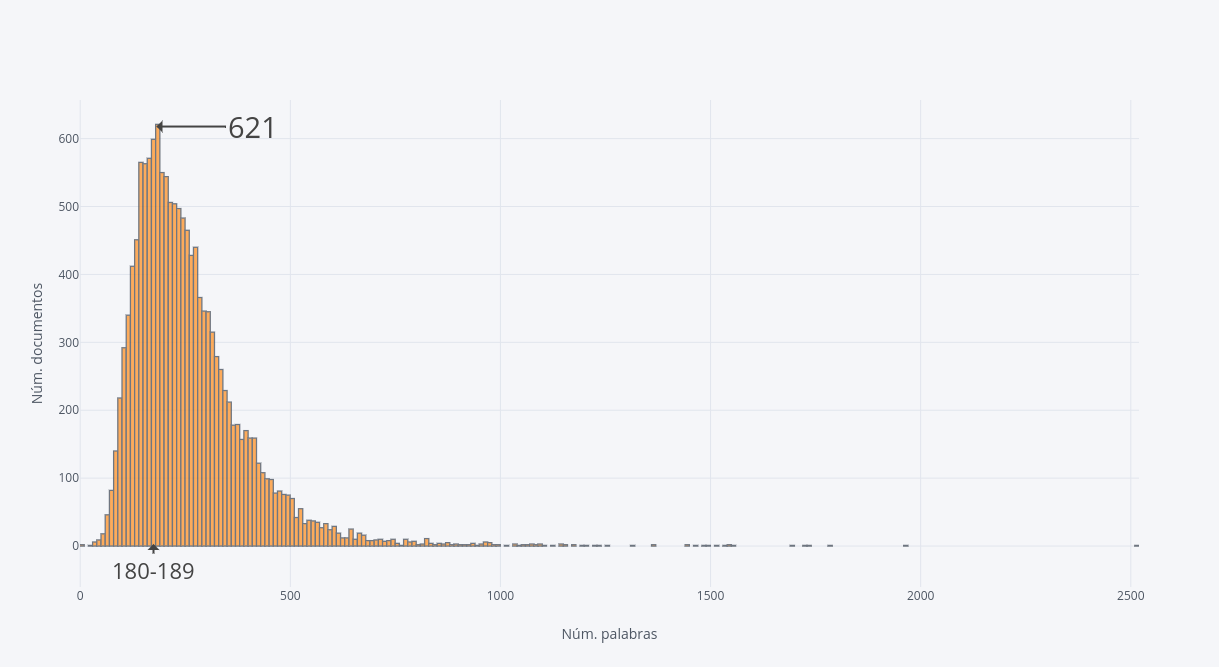
\includegraphics[width=1\textwidth]{imaxes/distTokensCine.png}
	\caption{Histograma de número de palabras por documento.}
	\label{dist_tokes_pelis}
\end{figure}

Está compuesto por un total de 5000 documentos con un alto número de oraciones por documento en comparación con el corpus TASS.

\begin{figure}[!ht]
	\centering
	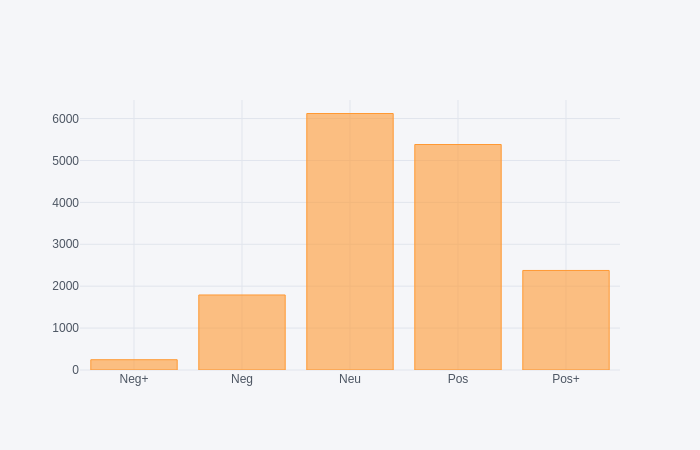
\includegraphics[width=0.75\textwidth]{imaxes/distCine.png}
	\caption{Distribución de la polarización.}
	\label{dist_pos_pelis}
\end{figure}

En este caso los usuarios de la red tienen tendencia a realizar críticas con valoraciones medias, encontrando muy pocos casos en los extremos.


\section{Machine learning}\label{sect:ML}

En las siguientes secciones comprobaremos el funcionamiento de los modelos para la clasificación de documentos del mismo dominio (TASS) y de distinto dominio (Cine).

Para establecer una línea base sobre la que probar  nuevos modelos o mejoras se ha realizado un entrenamiento con los parámetros por defecto de los modelos explicados en la sección \ref{alg}: MNB, LR, SVM, RF.


\subsection{Línea base}

\subsubsection{2 clases}

\begin{table}[H]
	\centering
	\begin{tabular}{|l|cccc|cccc|}
		\hline
		& \multicolumn{4}{c|}{TASS} & \multicolumn{4}{c|}{CINE} \\
		\cline{2-9}
		&    acc &     f1 &    mse &  recall & acc &     f1 &    mse &  recall \\
		\hline
		lr      &  77.17 &  81.07 &  22.83 &   77.54 &  51.48 &  33.48 &  48.52 &   79.37 \\
		ls      &  77.29 &  81.02 &  22.71 &   78.01 &  49.08 &  26.58 &  50.92 &   78.07 \\
		mb      &  79.97 &  \textbf{82.32} &  20.03 &   83.78 &  62.63 &  \textbf{63.90} &  37.37 &   72.04 \\
		rf      &  73.92 &  78.60 &  26.08 &   74.54 &  51.88 &  48.44 &  48.12 &   63.21 \\
		\hline
	\end{tabular}
	\caption{Resultados en \% entrenamiento para línea base.}
	\label{result-línea-base}
\end{table}

El modelo con mejores resultados es MNB, con un resultado de f1 de 82.32\% para el corpus TASS y un 63.90\% para el corpus de críticas de cine.


\subsubsection{3 clases}

\begin{table}[H]
	\centering
	\begin{tabular}{|l|cccc|cccc|}
		\hline
		& \multicolumn{4}{c|}{TASS} & \multicolumn{4}{c|}{CINE} \\
		\cline{2-9}
		&    acc &     f1 &    mse &  recall & acc &     f1 &    mse &  recall \\
		\hline
		lr      &  72.31 &  72.31 &   93.62 &   72.31 &  31.19 &  31.19 &  150.51 &   31.19 \\
		ls      &  72.40 &  72.40 &   93.34 &   72.40 &  28.63 &  28.63 &  162.97 &   28.63 \\
		mb      &  73.19 &  \textbf{73.19} &   81.34 &   73.19 &  37.35 &  \textbf{37.35} &  128.21 &   37.35 \\
		rf      &  68.05 &  68.05 &  110.27 &   68.05 &  32.78 &  32.78 &  137.66 &   32.78 \\
		\hline
	\end{tabular}
	\caption{Resultados en \% entrenamiento para línea base de 3 clases.}
	\label{result-línea-base-3-clases}
\end{table}

Al igual que en el caso de la clasificación binaria, el modelo con mejores resultados es el de Bayes con un 73.19\% para el TASS y un 37.35\% para las críticas de cine.

\subsubsection{5 clases}

\begin{table}[H]
	\centering
	\begin{tabular}{|l|cccc|cccc|}
		\hline
		& \multicolumn{4}{c|}{TASS} & \multicolumn{4}{c|}{CINE} \\
		\cline{2-9}
		&    acc &     f1 &    mse &  recall & acc &     f1 &    mse &  recall \\
		\hline
		lr      &  48.33 &  48.33 &  225.23 &   48.33 &  18.50 &  \textbf{18.50 }&  277.25 &   18.50 \\
		ls      &  48.09 &  48.09 &  240.97 &   48.09 &  16.09 &  16.09 &  307.73 &   16.09 \\
		mb      &  50.73 &  \textbf{50.73} &  200.21 &   50.73 &  16.47 &  16.47 &  302.59 &   16.47 \\
		rf      &  43.53 &  43.53 &  243.98 &   43.53 &  17.92 &  17.92 &  298.46 &   17.92 \\
		\hline
	\end{tabular}
	\caption{Resultados en \% entrenamiento para línea base de 5 clases.}
	\label{result-línea-base-5-clases}
\end{table}

En este caso las clasificaciones han bajado notablemente el resultado de la medida f1, obteniendo un 50.73\% para Bayes, pero en el caso del corpus de Cine las clasificaciones se encuentran por debajo de la aleatoriedad (20\% por ser 5 clases).

En el material anexo (sección \ref{analisis_bl_5}) se muestra un estudio sobre las causas de esta problemática.

\subsection{Experimentos de mejora Machine Learning}

Los experimentos han comenzado por un intento de mejora de los algoritmos de machine learning.

Como se menciona en \ref{sect:ML} para el establecimiento de la línea base se han utilizado los parámetros por defecto de los algoritmos. Para intentar encontrar una mejor combinación se ha realizado una validación cruzada de los siguientes parámetros:

\begin{itemize}
	\item Preprocesado de la negación (Verdadero o falso).
	\item Eliminación de carácteres repetido (Verdadero o falso).
	\item Rango de n-gramas (1 o 2).
	\item Tokenización o Stemming.
	\item Máximo número de iteraciones para SVM (1000, 2000, 1500).
	\item Máximo número de iteraciones para LR (100, 200, 500).
	\item Modificación del parámetro alpha para MB (1.0, 0.5 o 1.5).
	\item Número de estimadores para RF (10 o 100).
\end{itemize}

Además se ha repetido el proceso utilizando como preprocesador CountVectorizer y TFIDF.



\subsubsection{2 clases}

\begin{table}[H]
	\centering
	\begin{tabular}{|l|cccc|cccc|}
		\hline
		& \multicolumn{4}{c|}{CountVectorizer} & \multicolumn{4}{c|}{TF-IDF} \\
		\cline{2-9}
		&    acc &     f1 &    mse &  recall & acc &     f1 &    mse &  recall \\
		\hline
		lr      &  79.18 &  82.52 &  20.82 &   79.94 &  77.96 &  81.98 &  22.04 &   77.56 \\
		ls      &  78.24 &  81.70 &  21.76 &   79.24 &  79.97 &  82.87 &  20.03 &   81.63 \\
		mb      &  80.61 &  \textbf{82.90} &  19.39 &   84.20 &  79.18 &  \textbf{83.09} &  20.82 &   78.07 \\
		rf      &  75.14 &  78.85 &  24.86 &   77.30 &  73.89 &  78.03 &  26.11 &   75.75 \\
		\hline
	\end{tabular}
	\caption{Medias en \% entrenamiento para gridsearch con 2 clases.}
	\label{result-cv-kf}
\end{table}

En la tabla \ref{result-cv-kf} vemos que hemos conseguido mejorar la puntuación de todos los algoritmos. Cabe destacar el resultado del modelo de Bayes con un resultado cercano al 83\% en cualquiera de los métodos de selección de características.

\subsubsection{3 clases}

\begin{table}[H]
	\centering
	\begin{tabular}{|l|cccc|cccc|}
		\hline
		& \multicolumn{4}{c|}{CountVectorizer} & \multicolumn{4}{c|}{TF-IDF} \\
		\cline{2-9}
		&    acc &     f1 &    mse &  recall & acc &     f1 &    mse &  recall \\
		\hline
		lr      &  68.88 &  68.88 &  106.81 &   68.88 &  73.68 &  73.68 &   88.24 &   73.68 \\
		ls      &  67.84 &  67.84 &  111.58 &   67.84 &  74.95 &  \textbf{74.95} &   83.13 &   74.95 \\
		mb      &  70.12 &  \textbf{70.12} &  101.82 &   70.12 &  74.68 &  74.68 &   84.22 &   74.68 \\
		rf      &  66.63 &  66.63 &  111.79 &   66.63&  68.81 &  68.81 &  106.78 &   68.81 \\
		\hline
	\end{tabular}
	\caption{Medias en \% entrenamiento para gridsearch con 3 clases.}
	\label{result-cv-kf-3-clases}
\end{table}

En la tabla \ref{result-cv-kf-3-clases} vemos que el algoritmo tf-idf se comporta mejor ante la presencia de elementos con polaridad neutra. En este caso el modelo SVM es el de mayor puntuación.

\subsubsection{5 clases}

\begin{table}[H]
	\centering
	\begin{tabular}{|l|cccc|cccc|}
		\hline
		& \multicolumn{4}{c|}{CountVectorizer} & \multicolumn{4}{c|}{TF-IDF} \\
		\cline{2-9}
		&    acc &     f1 &    mse &  recall & acc &     f1 &    mse &  recall \\
		\hline
		lr      &  45.29 &  45.29 &  250.52 &   45.29 &  50.64 &  50.64 &  214.38 &   50.64 \\
		ls      &  44.68 &  44.68 &  284.19 &   44.68 &  50.70 &  \textbf{50.70} &  203.83 &   50.70 \\
		mb      &  46.41 &  \textbf{46.41} &  246.11 &   46.41 &  48.97 &  48.97 &  228.30 &   48.97 \\
		rf      &  39.57 &  39.57 &  278.27 &   39.57 &  45.08 &  45.08 &  241.49 &   45.08 \\
		\hline
	\end{tabular}
	\caption{Medias en \% entrenamiento para gridsearch con 5 clases.}
	\label{result-cv-kf-5-clases}
\end{table}

Como se muestra en la tabla \ref{result-cv-kf-5-clases} el algoritmo tf-idf es el que mayores puntuaciones obtiene, destacando el modelo SVM con una puntuación de 50.70\%.


\subsubsection{Conclusiones}

Si comparamos los dos métodos de preprocesado de textos que hemos utilizado vemos que el Tf-idf es el que mejores resultados obtiene para todos los casos de clasificación.

En cuanto a los mejores parámetros, hemos obtenido valores dispares en cuanto al parámetro estudiado de cada algoritmo, sin embargo en todos los casos se establecido como necesario el tratamiento de la negación, el uso de Stemming y el preprocesado de letras repetidas. En cuanto al rango de n-gramas en la mayoría de los casos se ha obtenido un valor de 1.

En cuanto a los modelos vemos que Bayes es el que mejor funciona para el CountVectorizer sin embargo en el otro caso es el modelo SVM el que mayor puntuación obtiene.

Con esto podemos deducir que deberíamos escoger Tf-idf como selector de características y el modelo SVM para realizar las clasificaciones.

En el material anexo se incluyen también resultados de adaptación al dominio para los modelos optimizados por grid search. Si comparamos los resultados de los clasificadores en el conjunto de test (tablas \ref{result-cv-test}, \ref{result-cv-test-3-clases} y \ref{result-cv-test-5-clases}) con los resultados en el dominio de críticas de cine (tablas \ref{result-cv-test-cine}, \ref{result-cv-test-3-clases-cine} y \ref{result-cv-test-5-clases-cine}) vemos que los modelos son tolerantes a la aparición de nuevos datos del mismo dominio pero su rendimiento baja notablemente en el otro caso. Esto se debe a que el algoritmo de selección de características está limitado a los elementos encontrados en el primer dominio y el resto de elementos del segundo dominio no serán tenidos en cuenta, provocando pérdida de información.


\section{Deep Learning}

En esta sección se mostrarán los resultados de los entrenamientos de modelos de Deep Learning.

Para estos casos se ha realizado una selección de parámetros manual sobre un modelo LSTM base, y posteriormente se han ejecutado el resto de algoritmos en la sección \ref{alg}. 

Todos los entrenamientos realizan 30 iteraciones (epochs).

\subsection{Selección de parámetros}

En esta sección mostraremos un ejemplo ilustrativo de cómo se ha iterado para la selección de parámetros de un modelo LSTM sobre el corpus TASS.

Este proceso se debe repetir para todas las distribuciones de clases y para todos los modelos.

\subsubsection{Base}

Este modelo se ha configurado con 64 neuronas en la capa oculta, y una activación RELU (fig. \ref{relu}) que limita las salidas de la capa a un valor entre 0 e infinito.

\begin{figure}[!ht]
	\centering
	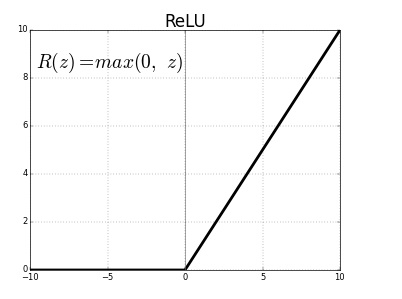
\includegraphics[width=0.75\textwidth]{imaxes/relu.jpg}
	\caption{Función de activación RELU}
	\label{relu}
\end{figure}

La gráfica \ref{evo_lstm_base} muestra la evolución de la pérdida en los conjuntos de entrenamiento y validación durante las 30 iteraciones del entrenamiento. Se han eliminado los valores con picos muy altos para facilitar la lectura.
Podemos ver que hacia el final del entrenamiento los valores de validación empiezan a divergir de los valores del conjunto de entrenamiento, esto es indicativo de que se comienza a producir un sobre entrenamiento.

\begin{figure}[H]
	\centering
	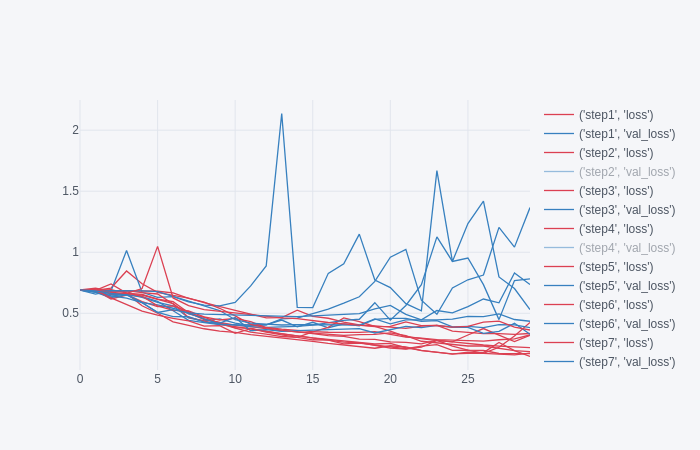
\includegraphics[width=0.75\textwidth]{imaxes/baselstm.png}
	\caption{Evolución entrenamiento modelo LSTM}
	\label{evo_lstm_base}
\end{figure}


El sobre entrenamiento generalmente es síntoma de un modelo excesivamente complejo y por lo tanto provoca un alto nivel de varianza ajustándose en exceso a los casos de entrenamiento. Para solucionar esto se ha probado un modelo más simple de 10 neuronas.

La evolución del modelo simplificado (\ref{simple}) muestra menos rasgos de sobre entrenamiento manteniendo más tiempo la tendencia a reducir la pérdida en el conjunto de validación.

\begin{figure}[H]
	\centering
	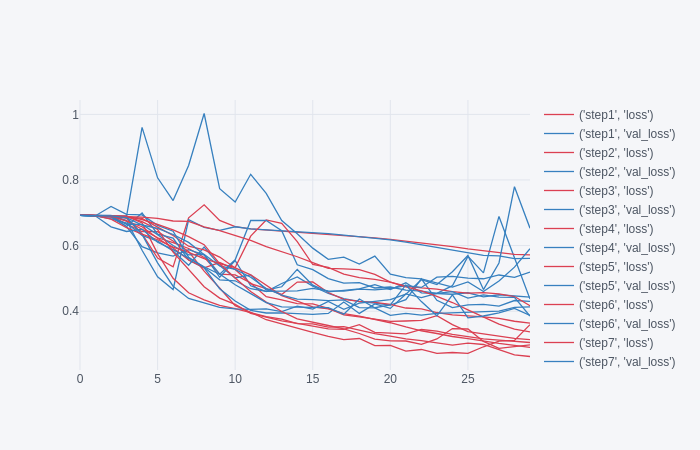
\includegraphics[width=0.75\textwidth]{imaxes/simple.png}
	\caption{Evolución entrenamiento modelo LSTM simplificado}
	\label{simple}
\end{figure}

Dado que la tendencia de este modelo es buena se han realizado pruebas configurando otros parámetros, como:

\begin{itemize}
	\item Dropout: Se introduce ruido sintético al modelo, apagando de forma aleatoria las neuronas durante el entrenamiento.
	\item Inicialización de pesos: Se cambia la inicialización de los pesos de las neuronas de la capa oculta, utilizando un tipo de inicialización conocida como Xavier initilization \cite{Glorot} o glorot normal, la cual asigna pesos de una distribución normal truncada centrada en el 0.
	\item Normalización de batch: Se normaliza la salida de la anterior capa de activación restando la media del batch y dividiendo por desviación típica. Con esto se consiguen entrenamientos más rápidos y menor varianza entre los resultados.
\end{itemize}

En la figura \ref{dropout02} vemos como han desaparecido los picos de las primeras iteraciones y parece que la evolución del entrenamiento es más adecuada, de forma que el modelo puede ser apto para seguir seleccionando mejores configuraciones.

\begin{figure}[H]
	\centering
	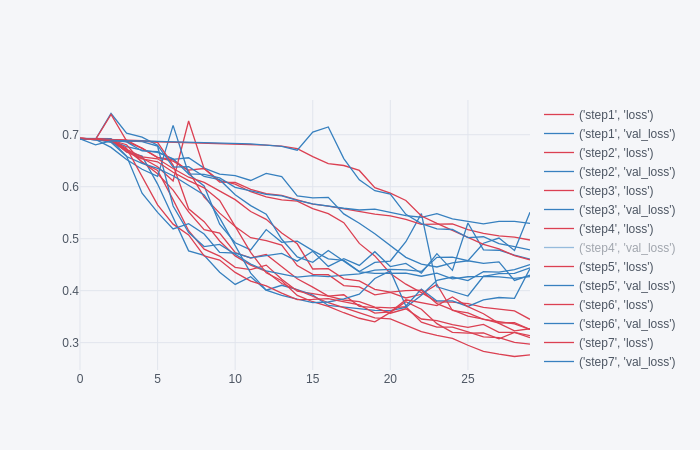
\includegraphics[width=0.75\textwidth]{imaxes/dropout0_2.png}
	\caption{Dropout con valor 0.2}
	\label{dropout02}
\end{figure}

En el siguiente experimento, aplicando inicialización Glorot (fig. \ref{glorot}) se aprecia se aprecia mayor uniformidad en la evolución si despreciamos los picos, que pueden ser debidos a una distribución poco favorable para este modelo. Sin embargo cuando aplicamos además la normalización de batch \ref{glorotbn}, aunque conseguimos eliminar los picos, vemos que se produce sobre entrenamiento en las primeras etapas.


\begin{figure}[H]
	\centering
	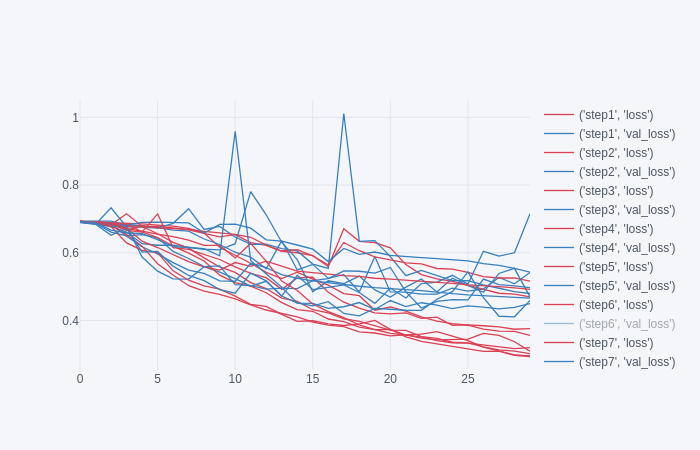
\includegraphics[width=0.75\textwidth]{imaxes/glorot.png}
	\caption{Inicialización Glorot más Dropout}
	\label{glorot}
\end{figure}

\begin{figure}[H]
	\centering
	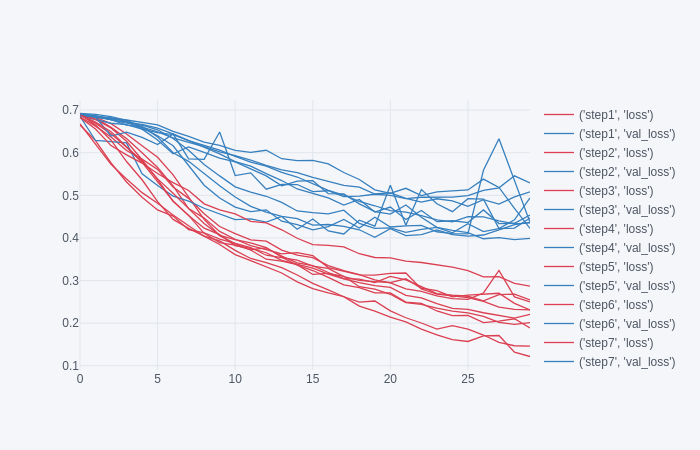
\includegraphics[width=0.75\textwidth]{imaxes/glorot_bn.png}
	\caption{Inicialización Glorot, dropout y normalización de batch}
	\label{glorotbn}
\end{figure}

Por lo tanto deberíamos quedarnos con el modelo con Dropout para seguir investigando ya que los otros parámetros no han dado resultados satisfactorios.



\subsection{2 clases}

\begin{table}[H]
	\centering
	\begin{tabular}{|l|cccc|cccc|}
		\hline
		& \multicolumn{4}{c|}{TASS} & \multicolumn{4}{c|}{CINE} \\
		\cline{2-9}
		&    acc &     f1 &    mse &  recall & acc &     f1 &    mse &  recall \\
		\hline
		base          &  80.21 &  80.34 &  19.79 &   94.84 &  49.54 &  31.90 &  50.46 &   71.72 \\
		simpler       &  81.42 &  83.21 &  18.58 &   87.47 &  56.46 &  60.81 &  43.54 &   63.16 \\
		dropout  &  81.84 &  84.24 &  18.16 &   84.86 &  58.92 &  69.71 &  41.08 &   60.61\\
		batch norm    &  82.27 &  85.12 &  17.73 &   82.95 &  57.80 &  \textbf{72.05} &  42.20 &   58.26\\
		glorot        &  81.56 &  84.97 &  18.44 &   80.59  &  58.26 &  66.35 &  41.74 &   61.95\\
		glorot\_wo\_bn  &  83.97 &  \textbf{85.80} &  16.03 &   88.24 &  56.58 &  60.20 &  43.42 &   63.79\\
		double        &  81.70 &  82.73 &  18.30 &   91.42 &  52.38 &  43.70 &  47.62 &   68.55\\
		conv          &  78.94 &  79.01 &  21.06 &   93.63 &  55.60 &  55.83 &  44.40 &   65.41\\
		conv2d        &  81.42 &  84.93 &  18.58 &   80.22 &  56.14 &  63.19 &  43.86 &   61.18\\
		bidirectional &  81.06 &  82.49 &  18.94 &   88.97 &  52.30 &  46.34 &  47.70 &   65.86 \\
		\hline
	\end{tabular}
	\caption{Resultados sobre el conjunto de test.}
	\label{test-dl-2-clases}
\end{table}

La tabla \ref{test-dl-2-clases} nos muestra el resultado de la clasificación del conjunto de test con los  modelos entrenados sobre todo el conjunto de entrenamiento. 

Vemos que los modelos con mejores resultados son los expuestos en la sección anterior, debido a que la optimización de parámetros ha permitido reducir la variación entre los resultados de las distintas particiones y por lo tanto son más robustos ante distintas distribuciones.

Cabe destacar el modelo con inicialización Glorot con 85.80\% en la medida f1, superando el 83.09\% obtenido como máximo en los modelos de Machine Learning.


\subsection{3 clases}

\begin{table}[H]
	\centering
	\begin{tabular}{|l|cccc|cccc|}
		\hline
		& \multicolumn{4}{c|}{TASS} & \multicolumn{4}{c|}{CINE} \\
		\cline{2-9}
		&    acc &     f1 &    mse &  recall & acc &     f1 &    mse &  recall \\
		\hline
		base          &  74.25 &  74.25 &  80.64 &   74.25 &  34.02 &  34.02 &  141.52 &   34.02\\
		simpler       &  75.25 &  75.25 &  76.65 &   75.25 &  33.58 &  33.58 &  143.10 &   33.58\\
		dropout  &  75.32 &  75.32 &  76.38 &   75.32 &  30.90 &  30.90 &  154.00 &   30.90\\
		batch norm    &  77.18 &  \textbf{77.18} &  68.93 &   77.18 &  34.24 &  34.24 &  140.64 &   34.24\\
		glorot        &  76.58 &  76.58 &  71.32 &   76.58 &  22.78 &  22.78 &  186.48 &   22.78 \\
		glorot\_wo\_bn  &  74.18 &  74.18 &  80.90 &   74.18 &  35.08 &  35.08 &  137.46 &   35.08\\
		double        &  74.12 &  74.12 &  81.17 &   74.12 &  31.48 &  31.48 &  151.96 &   31.48\\
		conv          &  73.25 &  73.25 &  77.64 &   73.25 &  35.74 &  \textbf{35.74} &  133.32 &   35.74\\
		conv2d        &  73.52 &  73.52 &  76.78 &   73.52 &  29.40 &  29.40 &  160.06 &   29.40\\
		bidirectional &  75.58 &  75.58 &  71.52 &   75.58 &  34.92 &  34.92 &  137.86 &   34.92\\
		\hline
	\end{tabular}
	\caption{Resultados sobre el conjunto de test.}
	\label{test-dl-3-clases}
\end{table}

En este experimento la mayor puntuación obtenida ha sido de 77.18\% por un modelo LSTM con normalización de batch, superando el 73\% obtenido con Machine Learning. 

La introducción de elementos neutros en el conjunto de datos produce picos de pérdida muy altos en los modelos, los cuales son suavizados gracias a la normalización de batch.

\begin{figure}[H]
	\centering
	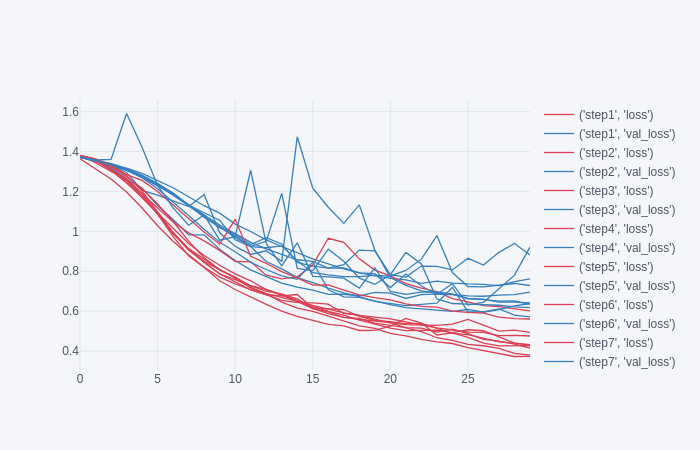
\includegraphics[width=0.75\textwidth]{imaxes/bn-3.png}
	\caption{Evolución modelo LSTM con normalización de batch.}
	\label{bn-3}
\end{figure}

\begin{figure}[H]
	\centering
	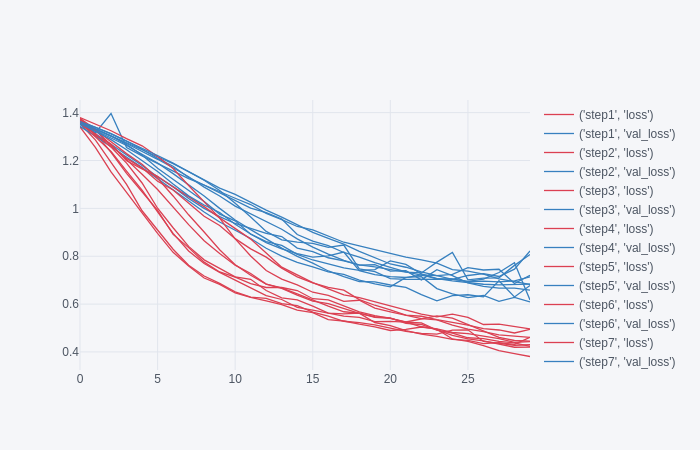
\includegraphics[width=0.75\textwidth]{imaxes/gn-3.png}
	\caption{Evolución modelo LSTM con normalización de batch e inicialización Glorot.}
	\label{gn-3}
\end{figure}

\begin{figure}[H]
	\centering
	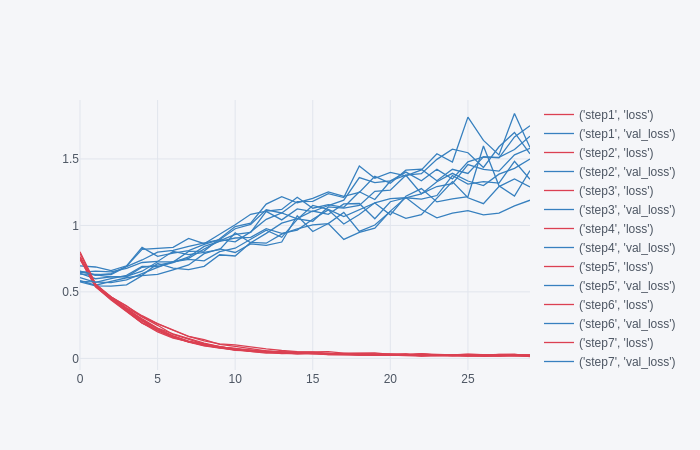
\includegraphics[width=0.75\textwidth]{imaxes/conv-3.png}
	\caption{Evolución modelo convolucional.}
	\label{conv-3}
\end{figure}

Si vemos las gráficas de evolución de los dos mejores modelos (figuras \ref{bn-3} y \ref{gn-3}) se observa una tendencia descendente que nos indica que podríamos obtener un mejor resultado afinando los parámetros o aumentando el número de iteraciones de entrenamiento. Por contra los modelos más complejos como el convolucional (fig. \ref{conv-3}) presentan sobre entrenamiento en fases tempranas del entrenamiento.

Los modelos complejos se comportan mejor en la clasificación con cambio de dominio.


\subsection{5 clases}

\begin{table}[H]
	\centering
	\begin{tabular}{|l|cccc|cccc|}
		\hline
		& \multicolumn{4}{c|}{TASS} & \multicolumn{4}{c|}{CINE} \\
		\cline{2-9}
		&    acc &     f1 &    mse &  recall & acc &     f1 &    mse &  recall \\
		\hline
		base          &  40.85 &  40.85 &  199.27 &   40.85 &  12.34 &  12.34 &  369.92 &   12.34 \\
		simpler       &  43.91 &  43.91 &  169.26 &   43.91 &  12.34 &  12.34 &  375.84 &   12.34 \\
		dropout   &  45.18 &  45.18 &  179.51 &   45.18  &   9.50 &   9.50 &  429.60 &    9.50\\
		batch norm    &  43.58 &  43.58 &  176.71 &   43.58 &   8.82 &   8.82 &  455.38 &    8.82\\
		glorot        &  45.51 &  45.51 &  201.60 &   45.51 &  11.76 &  11.76 &  382.44 &   11.76 \\
		glorot\_wo\_bn  &  43.05 &  43.05 &  176.31 &   43.05 &  13.24 &  13.24 &  357.64 &   13.24 \\
		double        &  41.85 &  41.85 &  142.38 &   41.85 &  21.80 &  \textbf{21.80} &  219.12 &   21.80\\
		conv          &  49.30 &  \textbf{49.30} &  214.77 &   49.30 &   9.14 &   9.14 &  443.42 &    9.14\\
		conv2d        &  43.11 &  43.11 &  182.97 &   43.11 &  11.26 &  11.26 &  400.44 &   11.26\\
		bidirectional &  45.51 &  45.51 &  182.37 &   45.51 &  12.00 &  12.00 &  396.64 &   12.00\\
		\hline
	\end{tabular}
	\caption{Resultados sobre el conjunto de test.}
	\label{test-dl-5-clases}
\end{table}

A pesar de que el mejor resultado en este experimento lo obtiene una red convolucional, vemos en la fig. \ref{conv-5} que durante su entrenamiento se ha producido un sobreentrenamiento.

Por otro lado los modelos Glorot con normalización de batch y sin ella presentan una tendencia a la baja como se ve en las figuras \ref{go-5} y \ref{gn-5} por lo que tenemos margen de mejora modificando hiperparámetros o ampliando el número de iteraciones hasta que se deje de apreciar una tendencia descendente en el entrenamiento.


\begin{figure}[H]
	\centering
	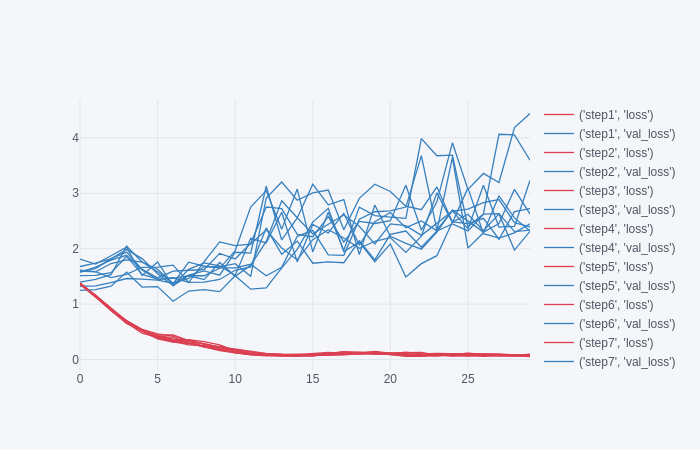
\includegraphics[width=0.75\textwidth]{imaxes/conv-5-clases.png}
	\caption{Evolución modelo convolucional.}
	\label{conv-5}
\end{figure}

\begin{figure}[H]
	\centering
	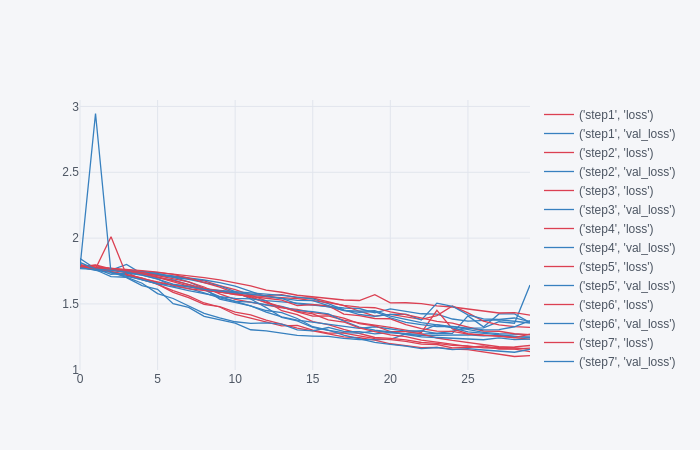
\includegraphics[width=0.75\textwidth]{imaxes/go.png}
	\caption{Evolución modelo LSTM con normalización de batch e inicialización Glorot.}
	\label{go-5}
\end{figure}

\begin{figure}[H]
	\centering
	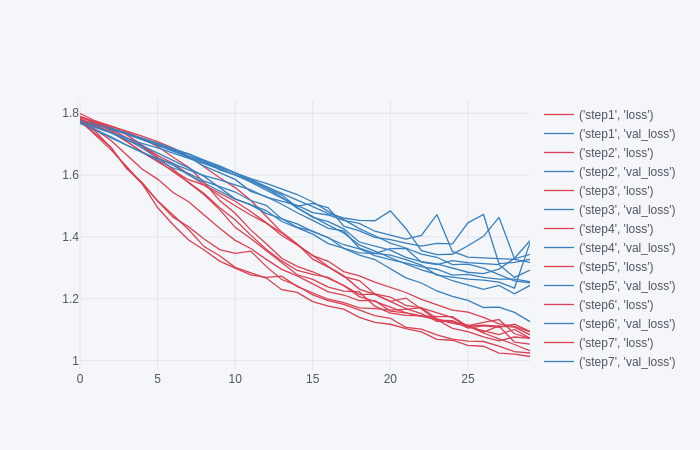
\includegraphics[width=0.75\textwidth]{imaxes/gnbn.png}
	\caption{Evolución modelo LSTM con inicialización Glorot.}
	\label{gn-5}
\end{figure}


\subsection{Conclusiones}

Tras analizar los resultados de las secciones anteriores podemos concluir que la complejidad del modelo no está directamente relacionada con su precisión ya que han sido los modelos más simples los que han obtenido mejor resultado. Destacando entre estos los modelos con inicialización Glorot, normalización del batch o una combinación entre ambos.

Las topologías complejas tienen tendencia a adaptarse muy rápido a los conjuntos de entrenamiento provocando un sobre entrenamiento. Esto puede ser debido a la simplicidad del conjunto de datos utilizado.

Podemos concluir que para la puesta en producción deberíamos utilizar los modelos de Deep Learning.

Además hemos demostrado que el corpus propuesto para los entrenamientos no nos garantiza los resultados finales, dado que desconocemos como van a ser los comentarios finales publicados en la aplicación. En estos experimentos hemos demostrado que si los documentos tienen mayor dimensionalidad que el corpus TASS se puede producir pérdida de información al cambiar de dominio y por lo tanto conseguir un peor rendimiento de los modelos.

Sería recomendable comenzar con una clasificación por umbrales, de forma que solo resulten clasificados automáticamente aquellos textos que tengan una probabilidad de pertenecer a una clase mayor a un tanto por ciento establecido entre la empresa y el cliente, además de ofrecer al usuario la posibilidad de clasificar su comentario, de esta forma dispondríamos de un corpus de comentarios con un valor establecido por humanos.

Cuando la aplicación cuente con un número de comentarios suficiente sería posible utilizarlos como corpus de entrenamiento.




